\mbox{$\displaystyle +\,$\,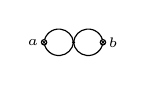
\begin{tikzpicture}[x=0.340cm, y=0.340cm, line width=0.420pt, baseline={([yshift=-0.6ex]0,0)}]
  \draw (-1.100,0.000) arc[start angle=186.026, end angle=353.974, radius=0.553];
  \draw (-1.100,0.000) arc[start angle=173.974, end angle=6.026, radius=0.553];
  \draw (1.100,0.000) arc[start angle=353.974, end angle=186.026, radius=0.553];
  \draw (1.100,0.000) arc[start angle=6.026, end angle=173.974, radius=0.553];
  \draw[fill=white] (-1.100,0.000) circle (0.100);
  \draw[line width=0.298pt] (-1.030,0.070) -- (-1.170,-0.070) (-1.030,-0.070) -- (-1.170,0.070);
  \draw[fill=white] (1.100,0.000) circle (0.100);
  \draw[line width=0.298pt] (1.170,0.070) -- (1.030,-0.070) (1.170,-0.070) -- (1.030,0.070);
  \fill (0.000,0.000) circle (0.064);
  \node[font=\tiny, inner sep=0pt, anchor=0] at (-1.290,0.000) {$a$};
  \node[font=\tiny, inner sep=0pt, anchor=180] at (1.290,0.000) {$b$};
\end{tikzpicture}}
\diagramgap
\mbox{$\displaystyle +\,2$\,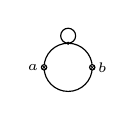
\begin{tikzpicture}[x=0.340cm, y=0.340cm, line width=0.420pt, baseline={([yshift=-0.6ex]0,0)}]
  \draw (-0.900,0.000) arc[start angle=180.000, end angle=360.000, radius=0.900];
  \draw (-0.900,0.000) arc[start angle=180.000, end angle=90.000, radius=0.900];
  \draw (0.900,0.000) arc[start angle=0.000, end angle=90.000, radius=0.900];
  \draw (0.000,0.900) arc[start angle=270.000, end angle=630.000, radius=0.280];
  \draw[fill=white] (-0.900,0.000) circle (0.100);
  \draw[line width=0.298pt] (-0.830,0.070) -- (-0.970,-0.070) (-0.830,-0.070) -- (-0.970,0.070);
  \draw[fill=white] (0.900,0.000) circle (0.100);
  \draw[line width=0.298pt] (0.970,0.070) -- (0.830,-0.070) (0.970,-0.070) -- (0.830,0.070);
  \fill (0.000,0.900) circle (0.064);
  \node[font=\tiny, inner sep=0pt, anchor=0] at (-1.090,-0.001) {$a$};
  \node[font=\tiny, inner sep=0pt, anchor=180] at (1.090,-0.001) {$b$};
\end{tikzpicture}}
